%% Run LaTeX on this file several times to get Table of Contents,
%% cross-references, and citations.

\documentclass[11pt]{book}
\usepackage{Wiley-AuthoringTemplate}
\usepackage[sectionbib,authoryear]{natbib}% for name-date citation comment the below line
%\usepackage[sectionbib,numbers]{natbib}% for numbered citation comment the above line

%%********************************************************************%%
%%       How many levels of section head would you like numbered?     %%
%% 0= no section numbers, 1= section, 2= subsection, 3= subsubsection %%
\setcounter{secnumdepth}{3}
%%********************************************************************%%
%%**********************************************************************%%
%%     How many levels of section head would you like to appear in the  %%
%%				Table of Contents?			%%
%% 0= chapter, 1= section, 2= subsection, 3= subsubsection titles.	%%
\setcounter{tocdepth}{2}
%%**********************************************************************%%

%\includeonly{ch01}
\makeindex

% Additional packages I use
\usepackage{breqn}

% My Macros
\newcommand{\set}[1]{\left \{ #1 \right \}}
\newcommand{\abs}[1]{\left | #1 \right |}
\newcommand{\encoding}[1]{\left \langle #1 \right \rangle}
\newcommand{\E}{\mathbb{E}}
\newcommand{\N}{\mathbb{N}}

% Image directory
\graphicspath{ {./images/} }

\begin{document}

\frontmatter
%%%%%%%%%%%%%%%%%%%%%%%%%%%%%%%%%%%%%%%%%%%%%%%%%%%%%%%%%%%%%%%%
%% Title Pages
%% Wiley will provide title and copyright page, but you can make
%% your own titlepages if you'd like anyway
%% Setting up title pages, type in the appropriate names here:

\booktitle{CPSC 421 \\ Introduction to Theory of Computing}

% \subtitle{Efficient Multirate Loss Models}

% \AuAff{Ioannis D. Moscholios\\ University of Peleponnese}

% \AuAff{Michael D. Logothetis\\ University of Patras}

%% \\ will start a new line.
%% You may add \affil{} for affiliation, ie,
%\authors{Robert M. Groves\\
%\affil{Universitat de les Illes Balears}
%Floyd J. Fowler, Jr.\\
%\affil{University of New Mexico}
%}

%% Print Half Title and Title Page:
\halftitlepage
\titlepage

%%%%%%%%%%%%%%%%%%%%%%%%%%%%%%%%%%%%%%%%%%%%%%%%%%%%%%%%%%%%%%%%
%% Copyright Page

% \begin{copyrightpage}{year}
% Title, etc
% \end{copyrightpage}

% Note, you must use \ to start indented lines, ie,
%
% \begin{copyrightpage}{2004}
% Survey Methodology / Robert M. Groves . . . [et al.].
% \       p. cm.---(Wiley series in survey methodology)
% \    ``Wiley-Interscience."
% \    Includes bibliographical references and index.
% \    ISBN 0-471-48348-6 (pbk.)
% \    1. Surveys---Methodology.  2. Social
% \  sciences---Research---Statistical methods.  I. Groves, Robert M.  II. %
% Series.\\

% HA31.2.S873 2004
% 001.4'33---dc22                                             2004044064
% \end{copyrightpage}

%%%%%%%%%%%%%%%%%%%%%%%%%%%%%%%%%%%%%%%%%%%%%%%%%%%%%%%%%%%%%%%%
%% Only Dedication (optional)

\dedication{To CPSC421 students}

\tableofcontents

%\listoffigures %optional
%\listoftables  %optional

%% or Contributor Page for edited books
%% before \tableofcontents

%%%%%%%%%%%%%%%%%%%%%%%%%%%%%%%%%%%%%%%%%%%%%%%%%%%%%%%%%%%%%%%%
%  Contributors Page for Edited Book
%%%%%%%%%%%%%%%%%%%%%%%%%%%%%%%%%%%%%%%%%%%%%%%%%%%%%%%%%%%%%%%%

% If your book has chapters written by different authors,
% you'll need a Contributors page.

% Use \begin{contributors}...\end{contributors} and
% then enter each author with the \name{} command, followed
% by the affiliation information.

%  \begin{contributors}
%  \name{Masayki Abe,} Fujitsu Laboratories Ltd., Fujitsu Limited, Atsugi, Japan

%  \name{L. A. Akers,} Center for Solid State Electronics Research, Arizona State University, Tempe, Arizona

%  \name{G. H. Bernstein,} Department of Electrical and Computer Engineering, University of Notre Dame, Notre Dame, South Bend, Indiana; formerly of
%  Center for Solid State Electronics Research, Arizona
%  State University, Tempe, Arizona
%  \end{contributors}

%%%%%%%%%%%%%%%%%%%%%%%%%%%%%%%%%%%%%%%%%%%%%%%%%%%%%%%%%%%%%%%%
% Optional Foreword:

% \begin{foreword}
% \lipsum[1-2]
% \end{foreword}

%%%%%%%%%%%%%%%%%%%%%%%%%%%%%%%%%%%%%%%%%%%%%%%%%%%%%%%%%%%%%%%%
% Optional Preface:

% \begin{preface}
% \lipsum[1-1]
% \prefaceauthor{}
% \where{place\\
%  date}
% \end{preface}

% ie,
% \begin{preface}
% This is an example preface.
% \prefaceauthor{R. K. Watts}
% \where{Durham, North Carolina\\
% September, 2004}

%%%%%%%%%%%%%%%%%%%%%%%%%%%%%%%%%%%%%%%%%%%%%%%%%%%%%%%%%%%%%%%%
% Optional Acknowledgments:

% \acknowledgments
% \lipsum[1-2]
% \authorinitials{I. R. S.}

%%%%%%%%%%%%%%%%%%%%%%%%%%%%%%%%
%% Glossary Type of Environment:

% \begin{glossary}
% \term{<term>}{<description>}
% \end{glossary}

%%%%%%%%%%%%%%%%%%%%%%%%%%%%%%%%
% \begin{acronyms}
% \acro{ASTA}{Arrivals See Time Averages}
% \acro{BHCA}{Busy Hour Call Attempts}
% \acro{BR}{Bandwidth Reservation}
% \acro{b.u.}{bandwidth unit(s)}
% \acro{CAC}{Call / Connection Admission Control}
% \acro{CBP}{Call Blocking Probability(-ies)}
% \acro{CCS}{Centum Call Seconds}
% \acro{CDTM}{Connection Dependent Threshold Model}
% \acro{CS}{Complete Sharing}
% \acro{DiffServ}{Differentiated Services}
% \acro{EMLM}{Erlang Multirate Loss Model}
% \acro{erl}{The Erlang unit of traffic-load}
% \acro{FIFO}{First in - First out}
% \acro{GB}{Global balance}
% \acro{GoS}{Grade of Service}
% \acro{ICT}{Information and Communication Technology}
% \acro{IntServ}{Integrated Services}
% \acro{IP}{Internet Protocol}
% \acro{ITU-T}{International Telecommunication Unit -- Standardization sector}
% \acro{LB}{Local balance}
% \acro{LHS}{Left hand side}
% \acro{LIFO}{Last in - First out}
% \acro{MMPP}{Markov Modulated Poisson Process}
% \acro{MPLS}{Multiple Protocol Labeling Switching}
% \acro{MRM}{Multi-Retry Model}
% \acro{MTM}{Multi-Threshold Model}
% \acro{PASTA}{Poisson Arrivals See Time Averages}
% \acro{PDF}{Probability Distribution Function}
% \acro{pdf}{probability density function}
% \acro{PFS}{Product Form Solution}
% \acro{QoS}{Quality of Service}
% \acro{r.v.}{random variable(s)}
% \acro{RED}{random early detection}
% \acro{RHS}{Right hand side}
% \acro{RLA}{Reduced Load Approximation}
% \acro{SIRO}{service in random order}
% \acro{SRM}{Single-Retry Model}
% \acro{STM}{Single-Threshold Model}
% \acro{TCP}{Transport Control Protocol}
% \acro{TH}{Threshold(s)}
% \acro{UDP}{User Datagram Protocol}
% \end{acronyms}

% \setcounter{page}{1}

% \begin{introduction}

% The word \textit {traffic} becomes \textit {teletraffic} in telecommunications, as communications becomes telecommunications to indicate technology use, e.g., conversation from some distance through phones or Internet. The term teletraffic covers all kinds of computer communication traffic and telecom traffic.  This book includes teletraffic loss models.
% \end{introduction}

\mainmatter

\chapter{Regular Languages}

\section*{Lecture 1: What is computation? Start of finite automata}

% TOOD: refactor lect1

\textbf{Exercises}:

\begin{enumerate}
    \item Sorting a list of names
    \item Given a polynomial, find its roots
    \item Given an integer, find its prime factors
\end{enumerate}

\textbf{Representation issues}: Encode input \& output

\textbf{Generic representation}:

\begin{definition}
    An \emph{alphabet} is a finite non-empty set. Typically denoted $\Sigma$ and $\Gamma$ (e.g. ASCII, Unicode: $\Sigma = \{0, 1\}$).
\end{definition}

\begin{definition}
    A \emph{string} is a finite sequence of zeros or more symbols from $\Sigma$ (e.g. text file, binary file).
\end{definition}

\begin{definition}
    $\Sigma^*$ is a set of all strings over alphabet $\Sigma$ (so $\Sigma^*$ is infinitely big).
\end{definition}

A problem is a mapping of strings to strings, e.g. for Ex. 3

\begin{verbatim}
    f("b") = "2, 3"
    f("30") = "2, 3, 5"
    f("28mT") = "error"
\end{verbatim}

\emph{Notice}: It must be a function.

\begin{definition}
    A \emph{decision problem} is a problem whose input is yes/no (accept/reject). E.g.

    \begin{enumerate}
        \item Is this list sorted?
        \item Given integers $(x, y)$. does x has a prime factor less than $y$?

        \begin{verbatim}
            f("35, 4") = "reject"
        \end{verbatim}
    \end{enumerate}
\end{definition}

\textbf{Important concept}: Decision problem $\equiv$ set of strings for which the function outputs ``accept''.

\begin{definition}
    A set of strings is called \emph{language}, so any set $S \in \Sigma^*$ is a language. So decision problems $\equiv$ languages
\end{definition}

\begin{equation*}
    \begin{aligned}
      L &= \set{S: s \text{ is a string of the form } s=\text{``p'' where p is a prime integer}}\\
      &\equiv \\
      f(s) &=
      \begin{cases}
        \text{``accept''} & \text{if s = ``p'' and p is a prime integer} \\
        \text{``reject''} & otherwise
      \end{cases}
    \end{aligned}
\end{equation*}

\section*{Lecture 2: Definition of finite automata}

Why?

\begin{itemize}
    \item To study the \emph{languages} related to F.A.
    \item
  \begin{enumerate}
    \item As a stepping-stone to richer computational models
    \item Useful background for NLP and compilers
    \item To understand regular expressions
  \end{enumerate}
\end{itemize}

\textbf{Informal definition}: A computational machine for a decision problem on any input string, either:

\begin{enumerate}
    \item outputs Accept and halts
    \item outputs Reject and halts
    \item runs forever
\end{enumerate}

In case 1 we say that machine \emph{accepts} $w$. The language \emph{accepted by machine} $M$.

\begin{equation*}
    L = \set{w \in \Sigma^*: M \text{ accepts } w}
\end{equation*}

\textbf{Theme}: Understand relationship between:

\begin{itemize}
    \item classes of machines
    \item classes of languages $\equiv$ classes of decision problems they can solve
    \item and their properties
\end{itemize}

\textbf{Finite Automata}

What is $L$ or $L(M)$?

Is it:

\begin{itemize}
    \item $\set{w: \text{either $w$ ends in 1 or \# 0s after the last 1 is even}}$
    \item $\{w: \text{$w$ contains a 1, and after the last 1, has even number of 0s}\}$
\end{itemize}

\begin{definition}
    A finite automaton is a 5-tuple $M=(Q, \Sigma, \delta, q_0, F)$ where

    \begin{itemize}
        \item $Q$ is a finite set (set of states)
        \item $\Sigma$ is a finite set (the alphabet)
        \item $\delta: Q \times E \rightarrow Q$ (the transition function)
        \item $q_0 \in Q$ (start state)
        \item $F \in Q$ (the accepting state)
    \end{itemize}
\end{definition}


\begin{definition}
    A F.A. $M$ accepts input string $w \in \Sigma^*$ if there exists a sequence $r_0, r_1, r_2, \cdots, r_n \in Q$ s.t.

    \begin{itemize}
        \item $r_0 = q_0$
        \item $r_i = \delta(r_{i-1}, w_i) \; \forall i = 1, \ldots, n$
        \item $r_n \in F$
    \end{itemize}

    Think of $r_0, \ldots, r_n$ as the sequence of states visited during the machine's computation.

    $L(M) = \{w \in \Sigma^*: M \text{ accepts } w\}$

    \begin{itemize}
        \item The language \underline{accepted} by $M$
        \item The language \underline{decided} by $M$
        \item The language \underline{recognized} by $M$
    \end{itemize}

\end{definition}

$L = \set{11011, 110011, 1100011, 11000011, \ldots}$

\textbf{Implicit Error States}: If $\delta$ is not fully specified, then we assume an implicit transition to an ``error state''.

\begin{definition}
    A \emph{regular language} is any language accepted by some Finite Automaton. The set of all regular languages is called the \emph{the class of regular languages}.
\end{definition}

\section*{Lecture 3: Nondeterministic finite automata}

\begin{definition}
    A regular language is any language $L$ s.t. some finite automaton accepts $L$.
\end{definition}

We will study operations on the class of regular languages.

For strings $x$, $y$ their concatenation is denoted $x \circ y$ or just $xy$.

\begin{definition}
    For languages $L_1$ and $L_2$
    \begin{align*}
        L_1 \circ L_2 &= \{x \circ y: x \in L_1 \text{ and } y \in L_2\}
    \end{align*}
\end{definition}

If $L_1$ and $L_2$ are regular, is $L_1 \circ L_2$ also?

$L_1 = \{Messi\}$

$L_2 = \{Alba\}$

$L_1 \circ L_2 = \{MessiAlba\}$

\begin{unnumfigure}
    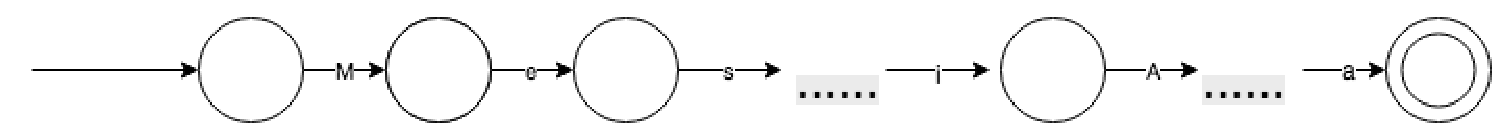
\includegraphics[scale=0.4]{lect3_img1.eps}
\end{unnumfigure}

$M_3$ accepts $L_1 \circ L_2$ $\Rightarrow$ $L_1 \circ L_2$ is regular.

\begin{definition}
    A \emph{non-deterministic finite automaton} is a 5-tuple $M = (Q, \Sigma, \delta, q_0, F)$ s.t.

    \begin{itemize}
        \item $Q, \Sigma, q_0, F$ are the same
        \item $\delta: Q \times (\Sigma \cup \{\epsilon\}) \rightarrow 2^Q$
        \begin{itemize}
            \item $\delta (q, s)$ is a subset of $Q$
        \end{itemize}
    \end{itemize}
\end{definition}

For a set $S$, $2^S$ is called the \emph{power set} of $S$. It contains all subsets of $S$.

$2^{\set{a, b}} = \set{\emptyset, \set{a}, \set{b}, \set{a, b}}$

\begin{definition}
    The NFA $M$ accepts the string  $w = w_1w_2 \ldots$ if there exists a string $y = y_1y_2 \ldots y_m \in (\Sigma \cup \set{\epsilon})^*$  and a sequence $r0, r_1, \ldots r_m \in Q$ such that:

    \begin{itemize}
        \item $w = y_1 \circ y_2 \circ \cdots \circ y_m$
        \item $r_0 = q_0$
        \item $r_i \in \delta (r_{i-1}, y_i) \text{ for } i = 1, \cdots, m$
        \item $r_m \in F$
    \end{itemize}
\end{definition}

Input string: $w = 00$

$y = \epsilon 00$, $r = q_0q_1q_2q_1$

$\delta(q_0, \epsilon) = \set{q_1, q_3}$

\section*{Lecture 4: Converting NFA-DFA, Operations on regular languages}

Language accepted by DFAs = Language accepted by NFAs = Regular Languages

Important properties of Regular Languages i.e. \emph{closure} properties. These are much easier to prove using NFAs.

\begin{theorem}[1.25 and 1.45 in texts]
    If $A$ and $B$ are regular, so is $A \cup B$ $\{x: x \in A \text{ or } x \in B\}$.
\end{theorem}

\begin{proof}
    The slide shows there is an NFA that accepts $A \cup B$.

    By theorem 1.39, $A \cup B$ is a regular language.
\end{proof}

\begin{theorem}
    Let $A$ and $B$ be regular. Then so are:

    \begin{itemize}
        \item Concatenation: $A \circ B = \set{x \circ y: x \in A, y \in B}$
        \item Star: $A^* = \set{x_1 \circ x_2 \circ \cdots \circ x_k: \text{ each } x_i \in A \text{ and } k \geq 0}$
        \item Complement: $\Sigma^* \diagdown A = \set{x: x \notin A}$
    \end{itemize}

    \emph{Note}: $\Sigma$ is in $A*$ $\rightarrow$ start state must be an accepting state
\end{theorem}

\begin{proof}
    (Theorem 1.39 and 1.40)

    \emph{Main claim}: Let $M = (Q, \Sigma, \delta, q_0, F)$ be an NFA. Let $L$ ba a language accepted by $M$. We can construct a DFA $M' = (Q', \Sigma, \delta', q_0, F)$ that also accepts $L$ (so $M$ and $M'$ are equivalent).

    First we need to define $\epsilon$-closure. For any set $S \subseteq Q$, let \emph{$E(S)$} be the set of all states in $Q$ that can be reached by following any number of $\epsilon$-transitions.

    \emph{Back to proof}:

    \begin{itemize}
        \item The states $Q' = 2^Q$ $\set{S: S \subseteq Q}$
        \item Accepting state $F' = \set{S \subseteq Q: \text{ any state in $S$ is an accepting state }} = \set{S \subseteq Q: S \cap F \neq \emptyset }$
    \end{itemize}

    \emph{Start state}: $q_0' = E(\set{q_0})$

    \emph{Transition function $\delta'$}:

    If NFA could be in states $S$, next input symbol is a, what states could it be in next?
    \begin{itemize}
        \item First, it could follow any $\epsilon$-transition, so could move to any state in $E(S)$.
        \item Next, unite $E(S) = \set{S_1, \ldots, S_n}$ could move to any state in $\delta(S_1, a) \cup \delta(S_2, a) \cup \ldots = \cup_{S \in E(S)} \delta(S, a)$.
        \item Again, it can follow any $\epsilon$-transitions
    \end{itemize}

    Final definition: $\delta'(S, a) = E(\cup_{S \in E(S)} \delta(S, a))$.
\end{proof}

\section*{Lecture 5: Regular expressions, Non-regular languages}

We will ``show'': A language is a regular iff it can be described by a \emph{regular expression}.

$R$:

\begin{itemize}
    \item $0^*1^*$
    \item $\Sigma^*001\Sigma^*$
    \item $(\Sigma\Sigma)^*$
    \item $\Sigma^*1\Sigma^*1\Sigma^*$
\end{itemize}

\emph{Shorthand}: $\Sigma = (a_1|a_2|\ldots|a_k) \text{ where } \Sigma  = a_1a_2\ldots a_k$

$L(R)$: the set of strings generated by regular expression $R$.

\begin{itemize}
  \item $\set{0^i1^j: i, j \geq 0}$
  \item \{all strings containing $001$ as a substring\}
  \item \{all strings of even length\}
  \item $\set{w: w \text{ contains at least three 1s}}$
\end{itemize}

$\Leftarrow$: Any regular expression can be converted into an equivalent NFA.

$\Rightarrow$: Idea: generalize NFAs by allowing arbitrary R.Es as labels on their transitions. Keep simplifying.

\emph{Limits to the power of Finite Automata}

Can any language be described by a F.A?

\begin{example}
    Suppose $L$ is a finite language (i.e. $L$ is finite). Is $L$ regular? Yes

    Why? Suppose $L = \set{x_1, \ldots, x_n}$.

    We can define $L_i = \set{x_i}$. This is regular. We know $L_1 \cup L_2$ is regular, so $L_1 \cup L_2 \cup \ldots \cup L_n$ is regular.

    This fails if $L$ is infinite because we could get an ``Infinite Automaton''.
\end{example}

\begin{example}
    Suppose $L$ is regular. Define $L^2 = \set{xy: x \in L \text{ and } y \in L}$

    This is regular: it is $L \circ L$.
\end{example}

\begin{example}
    $L^{dup} = \set{xx: x \in L}$

    Is this regular? It depends $\ldots$

    If $L$ is finite, $L^{dup}$ is finite, hence regular.

    If $L = L(1^*)$, then $L^{dup} = \set{1^{2i}: i \geq 0} = L((11)^*)$

    If $L = \Sigma^*$, $L^{dup} = \set{xx: x \in \Sigma^*}$. Is this regular?

    \emph{Intuitive argument}: $\set{xx: x \in \Sigma^*}$ is not regular.

    \begin{itemize}
        \item With a F.A. its states are its ``memory''.
        \item Any F.A. accepting $L^{dup}$ ``must remember'' the first half to compare to the second half.
        \item So F.A. must remember arbitrary large information, but it can't.
    \end{itemize}
\end{example}

\emph{Idea about finite automaton}:

\begin{unnumfigure}
    \includegraphics[scale=0.25]{lect5_img1}
\end{unnumfigure}

\begin{itemize}
    \item $\rightarrow$ ``computation path'', transitions followed when processing input
\end{itemize}

If input is very long, this computation path must have a \emph{cycle}.

\section*{Lecture 6: Pumping lemma: Proving languages are not regular}

$L = \set{w: w \text{ has a equal \# of occurrences of substrings 01 and 10 }}$

This \emph{is} a regular, surprisingly (Ex 1.48).

\begin{unnumfigure}
    \includegraphics[scale=0.2]{lect6_img1}
\end{unnumfigure}

Give the DFA a long input string $w$. \emph{Computation path on input $w$} must contain a cycle. Let $x$ be the part of input that was processed before arriving at $q$. While going round cycle, read $y$ from input. After cycle, we read $z$ from input.

What if input were $xyyz$. The DFA also accepts; we just travel cycle twice.

\emph{Message}: If $L$ is regular, then for a sufficiently long string $w \in L$, we can repeat its special substring $y$, to get another string in $L$.

\emph{Refinement of Message}: Let $p$ = \# states of DFA. If $|w| \geq p$ then computation path has length $\geq p + 1$. By Pigeonhole Principle, a cycle exists. So we can assume $\abs{xy} \leq p$. That's enough to get a cycle.

\emph{Important Point}:

\begin{itemize}
  \item We can (usually) use Pumping Lemma to prove that a language is not regular by proving that it satisfies the negation of Pumping Condition.
  \item We \emph{cannot} use P.L to prove that a language is regular.
\end{itemize}

How to negate a statement with logical quantifiers:

\begin{itemize}
  \item $\exists x$ s.t. $f$ becomes $\forall x$, NOT $f$
  \item $\forall x$, $g$ becomes $\exists x$ s.t. NOT $g$
\end{itemize}

\backmatter

\chapter{Context-Free Languages}

\section*{Lecture 7: Push down automata}

\begin{itemize}
    \item Only read input once, left to input
    \item Only finite memory
\end{itemize}

Basically, NFA with infinite stack (DFA + stack).

It turns out:
\begin{itemize}
    \item NFA + queue $\equiv$ Turing Machine
    \item NFA + 2 stacks $\equiv$ Turing Machine
\end{itemize}

Transitions of NFA now become: If in state $q$ and see symbol $a$ (or $\epsilon$) in input, and see $\sigma$ on stop of stack (or ignore it) then pop it, push $c$ onto the stack (or $\epsilon$) goto state $q'$ (if no transition $\rightarrow$ implicit reject).

\begin{example}[2.14 in text]
    $L = \{0^n1^n: n \geq 0\}$ This is not regular.
\end{example}

Exercise: $L = \{a^i b^j c^k: i, j, k \geq 0 and i = j \text{ or } i = k\}$

Hints:

\begin{enumerate}
  \item Need nondeterminism
  \item $L$ contains both $aabccc$ $(i = k)$ and $aabbc$ $(i = j)$
\end{enumerate}

\chapter{The Church-Turing Thesis}

\section*{Lecture 13: Examples of Multitape and Nondeterministic TMs}

\begin{example}
    $L = \{x\#x : x \in \Sigma^*\}$

    Let's do an implementation-level description of a multi-tape TM for $L$. Our original TM took time $\Theta(n^2)$ for inputs of length $n$.

    \begin{enumerate}
        \item Scan head 1 to the right until it reads a \#. Move Right. (Second head is still at start of tape 2)
        \item Repeatedly read symbol from tape 1, write it to tape 2, move both heads right, until seeing a blank on tape 1. Now second half of input is on tape 2.
        \item Move both heads left until they reach start of tapes (possibly using \$ back to find start of tape). Replace \# by $\textvisiblespace$ while doing so.
        \item Repeat until $\textvisiblespace$ on both tapes. If symbols differ, reject. Else, move both heads right.
    \end{enumerate}

    The multi-tape TM runs in $\Theta(n)$ time!
\end{example}

Last time: Configuration of TM, $aqb$, $a, b \in \Gamma^*$, $q \in Q$

Acceptance of a NTM: Input string is accepted if $\exists$ configurations $c_0, c_1, \ldots, c_k$ where:

\begin{itemize}
    \item $c_0 = q_{start} \; w$
    \item $c_i \Rightarrow c_{i+1}$ ($c_{i+1}$ is a possible configuration from $c_i$ following the transition function $\delta$)
    \item $c_k$ is on the accepting state
\end{itemize}

i.e. in a tree of configs, is there an accepting state:

\begin{enumerate}
    \item $w$ is accepted: any node in tree is an accepting state
    \item $w$ is explicitly rejected: the tree is finite, but yet no node is accepting config i.e. all leaves are rejection configs
    \item The NTM runs forever on $w$: the tree is infinite, but no node is accepting config
\end{enumerate}

\begin{definition}
    A NTM is a decider if for all inputs, case 1 or 2 happens.
\end{definition}

Example of NTMs: Let $L_1$, $L_2$ be recognizable languages. Let $M_i$ be a TM that recognizes $L_i$.

\emph{Claim}: $L_1 \cup L_2$ is recognizable. A cheat! Let's use nondeterminism.

\begin{definition}
    Define a NTM $M$ as follows:

    \begin{itemize}
        \item Nondeterministically choose to do one of the following:
        \begin{itemize}
            \item Run $M_1$
            \item Run $M_2$
        \end{itemize}
      \end{itemize}
\end{definition}

\emph{Claim}: $M$ recognizes $L_1 \cup L_2$.

\begin{proof}
    Suppose $w \in L_1 \cup L_2$. Say $w \in L_2$. Then the branch of tree simulating $M_i$ will accept. So $M$ is in case 1, and accepts. If $w \notin L_1 \cup L_2$, then both $M_1 \& M_2$ either run forever or reject. So $M$ is in either case 2 and case 3. So $M$ does not accept $w$.
\end{proof}

\begin{theorem}
    Given a NTM $M$, we can construct a DTM $M$ s.t. $L(M) = L(M')$.
\end{theorem}

\begin{theorem}
    If $M$ is a NTM decider, then we can make $M'$ a decider as well.
\end{theorem}

Using Theorem, we get a DTM $M'$, completing proof of claim 1.

\chapter{Decidability}

\section*{Lecture 15: Encodings, Universal Turing Machine, Countable Sets}

\emph{Encodings} \textsf{TM} input is always a string. Need to represent other objects as strings. Same as ``serialization'', e.g. JSON. If we have an object $O$ (e.g. a graph) then $\encoding{O}$ represents it as a string. Assume TMs can do serialization.

We can also represent TMs as strings.

\begin{equation*}
    HALT_{\text{TM}} = \set{\encoding{M, w}: M \text{ is a TM, } w \in \Sigma^* \text{, and } M \text{ halts on input} w} \tag{The Halting Problem}
\end{equation*}

\begin{equation*}
    A_{\text{TM}} = \set{\encoding{M, w}: M \text{ accepts } w}
\end{equation*}

What strings are in $A_{\text{TM}}$!

\begin{itemize}
    \item If $x$ is of form $\encoding{M, w}$
\end{itemize}

\section*{Lecture 16: Undecidability of ATM}

$A$ =  statement on the left is False. $B$ = statement on the right is True. If $A$ is true $\Rightarrow$ B is false $\Rightarrow$ $A$ is false.

$\set{0, 1}^* = \set{\epsilon, 0, 1, 00, 01, \ldots}$ countable

$B = \set{0000\ldots, 111\ldots, 010101\ldots}$

Why not apply diagonalization to $\set{0, 1}^*$?

We need to define $a_n$. Each row $f(n)$ has finite length. If $f(n)$ has finite length $\geq n$, then $a_n$ is undefined.

$2^{\Sigma^*}$ is uncountably infinite.

There are many TMs

\begin{description}
    \item $\Rightarrow$ countably many decidable many languages (each decided by some TM)
    \item $\Rightarrow$ countably many recognizable languages (each recognized by some TM)
\end{description}

\chapter{Reducibility}

\section*{Lecture 17: Reductions}

Recall:

\begin{itemize}
    \item $A_{\text{TM}} = \set{\encoding{M, w} : M \text{ accepts } w}$
    \item $HALT_{\text{TM}} = \set{M \text{ halts on } w}$
\end{itemize}

\begin{theorem}
    $HALT_{\text{TM}}$ is undecidable.
\end{theorem}


\begin{proof}
    Last time showed that $A_{\text{TM}}$ is undecidable. Show that $A_{\text{TM}} \leq_{T} HALT_{\text{TM}}$. Suppose we have a TM $R$ that decides $HALT_{\text{TM}}$. Then we want to create a TM $S$ that decides $A_{\text{TM}}$.

  Design $S$: On input $x$,

  \begin{enumerate}
        \item Reject if $x$ not in form of $\encoding{M, w}$.
        \item Run $R$ on input $\encoding{M, w}$.
        \item If $R$ accepts, (we know $M$ halts on input $w$), simulate $M$ on input $w$. Accept if $M$ accepts, reject if $M$ rejects. Else ($M$ runs forever on input $w$). Reject. ($M$ does not accept $w$)
  \end{enumerate}

  So $S$ is a decider for $A_{\text{TM}}$. Contradiction!
\end{proof}

\emph{Claim}: Suppose $L$ and $\overline{L}$ are both recognizable, then $L$ is decidable (and so is $\overline{L}$.

\begin{proof}
    Let $M_1$ be TM that recognizes $L$. Let $M_2$ be TM that recognizes $\overline{L}$. Design a new TM $M_3$ as follows: on input $x$,

  \begin{enumerate}
        \item In parallel simulate both $M_1$ and $M_2$.
        \item If $M_1$ halts and accepts then $M_3$ accepts.
        \item If $M_2$ halts and accepts then $M_3$ rejects.
  \end{enumerate}

    Suppose $x \in L$. Then $M_1$ eventually accepts $x \Rightarrow M_3$ accepts $x$. $x \notin L$, then $M_2$ eventually accepts $x \Rightarrow M_3$ rejects $x$. So $M_3$ decides $L$.
\end{proof}

\begin{corollary}
    $\overline{A_{\text{TM}}}$ is not recognizable.
\end{corollary}

\begin{proof}
    If it was recognizable, Claim should imply $A_{\text{TM}}$ is decidable!
\end{proof}

\section*{Lecture 18: More reductions}

\begin{equation*}
    E_{TM} = \{\langle N \rangle : N \text{ is a TM s.t. } L(N) = \emptyset\}
\end{equation*}

\begin{theorem}[Sipser 5.1]
    $E_{TM}$ is undecidable.
\end{theorem}

\begin{proof}
    We know $A_{\text{TM}}$ is undecidable. We want to prove $A_{\text{TM}} \leq_{T} E_{TM}$. Then we can conclude that $E_{\text{TM}}$ is undecidable.
    How to do reduction? Assume that $R$ is a (hypothetical) TM solving $E_{\text{TM}}$. We must somehow construct a TM $S$ that decides $A_{TM}$. $A_{TM} = \{\encoding{M, w}: M \text{ accepts } w\}$.

    \emph{Design of $S$}:

    On input $X$:
    \begin{enumerate}
        \item If $x$ is not of form $\encoding{M, w}$, reject.
        \item Construct description of $N$ like this:

        Let $N$ be TM: On input $y$, (ignore input), simulate $M$ on input $w$:

        \begin{enumerate}
            \item If $M$ accepts $N$ accepts.
            \item If $M$ rejects $N$ rejects.
        \end{enumerate}

        \item Run $R$ on input $\encoding{N}$.
        \item Accept if $R$ rejects; reject if $R$ accepts.
    \end{enumerate}

    $S$ is a decider since $R$ is.

    \emph{What is $L(N)$}:

    Case 1: $M$ accepts $w$. Then $L(N) = \Sigma^*$.

    Case 2: $M$ does not accept $w$:

    \begin{enumerate}[2a.]
        \item $M$ rejects $w$. Then $N$ rejects all inputs, so $L(N) = \emptyset$.
        \item $M$ runs forever on input $w$. Then $N$ runs forever on all inputs, so $L(N) = \emptyset$.
    \end{enumerate}

    \emph{Analysis}:

    In Case 1, then $R$ rejects $\encoding{N}$, so $S$ accepts ($M$ accepts $w$). Otherwise, $L(N) = \emptyset$, so $R$ accepts $\encoding{N}$, so $S$ rejects.
\end{proof}

\begin{equation*}
    REGULAR_{\text{TM}} = \set{\encoding{N} : N \text{ is a TM s.t. } L(N) \text{ is regular}}
\end{equation*}

\begin{proof}
    We know $A_{\text{TM}}$ is undecidable. We want to prove $A_{\text{TM}} \leq_{T} E_{\text{TM}}$. Then we can conclude that $REGULAR_{\text{TM}}$ is undecidable.

    \emph{What is $L(N)$}:

    Case 1: $M$ accepts $w$. Then $L(N) = \set{0^n1^n : n \in \N}$ (NOT REGULAR!).

    Case 2: $M$ does not accept $w$:

    \begin{enumerate}[2a.]
        \item $M$ rejects $w$. $L(N) = \emptyset$ is regular.
        \item $M$ runs forever on input $w$. $L(N) = \emptyset$ is regular.
    \end{enumerate}

    \emph{Analysis}:

    If $M$ accepts $w$, then $L(N)$ is not regular, so $R$ rejects, so $S$ accepts. Otherwise, $L(N) = \emptyset$, so $R$ accepts $\encoding{N}$, so $S$ rejects.
\end{proof}


\chapter{Time Complexity}

\section*{Lecture 19: Definition of P, EXP}

\begin{definition}
    The running time of a (deterministic) TM is a function $f:\N \rightarrow \N$ given by $f(n) = \max\limits_{\substack{x \in \Sigma^* \\ \abs{x} = n}}^{}$ (\# of steps of $M$ on input $x$).
\end{definition}


Typically we assume $M$ is a decider now.

A class of languages defined by some resource constraint is called a \emph{complexity class}.

\begin{definition}
    \begin{dmath*}
        TIME(t(n)) = \set{\text{language } L : \text{ there exists a TM with running time } O(t(n))}
    \end{dmath*}
\end{definition}

\begin{definition}
    $P = \bigcup\limits_{c>0}^{} TIME(n^c)$
\end{definition}

\begin{definition}
    $EXP = \bigcup\limits_{k \geq 0} TIME(2^{n^k})$ or $EXPTIME$
\end{definition}

\begin{equation*}
    3COLORMAP \in TIME(4^n) \subseteq EXP
\end{equation*}

\section*{Lecture 20: Time hierarchy theorem, Definition of NP}

\begin{definition}
    $EXP = \bigcup\limits_{k \geq 1} TIME(2^{n^k})$ and $P = \bigcup\limits_{c > 0} TIME(n^c)$
\end{definition}

\emph{Claim}: $P \subseteq EXP$

Why? Because $n^c = O(2^n)$.

\begin{theorem}[Time Hierarchy Theorem]
    Let $f:\N \rightarrow \N$ be ``reasonable'', and $f(n) = \Omega(n \log{n})$. Then $TIME(f(n)) \not\subseteq TIME(f(4n)^4 \text{ or } f(n)^2)$
\end{theorem}

\begin{example}
    Let $f(n) = n^c, TIME(n^c) \not\subseteq TIME(n^{4c}) \; \forall c > 1$.
\end{example}

\begin{corollary}
    $TIME(n^c) \not\subseteq TIME(2^n) \;\forall c > 1$
\end{corollary}

\begin{corollary}
    $P \not\subseteq TIME(2^n) \subseteq EXP$
\end{corollary}

\emph{Claim}: $P \subseteq NP$

Open Question 1: Is $P \neq NP$?

Open Question 2: Is $N \neq EXP$?


\begin{theorem}
    Either Question 1 or Question 2 is True.
\end{theorem}

Why? Because $P \neq EXP$. It is believed that $P \neq NP \neq EXP$.

\begin{theorem}[Sipser 7.20]
    The following are equivalent:

    \begin{enumerate}
        \item $L \in NP$
        \item There exists a deterministic, polynomial time TM V and a constant $c$, such that $L = \set{x \in \Sigma^* \; \exists y \in \Sigma^* \text{ such that } \abs{y} \leq \abs{x}^c \text{ and } V \text{ accepts } (x, y)}$
    \end{enumerate}
\end{theorem}

$V$ is called a ``verifier''. $y$ is called a ``certificate''.

\section*{Lecture 21: Polytime Reductions, 2 Definitions of NP, SAT}

\begin{equation*}
    L = \set{x : \exists y, |y| \leq \abs{x}^c, V \text{ accepts } x, y}
\end{equation*}

Must show:

\begin{enumerate}
    \item If $G$ is 3-colourable, then $\exists y$ s.t. $V$ accepts $x, y$, y should be a valid 3-colouring.
    \item If $G$ is \underline{not} 3-colourable, then $\forall y$, $V$ will not accept $x, y$.
    \item $V$ runs in polynomial. Runtime is $O(\abs{V} + \abs{E})$ in our example. + decoding time, which is polynomial in input size.
\end{enumerate}

Runtime of $M$ is, let $n = \abs{x}$: $\underbrace{(2^{n^c})}_{\text{if } \abs{\Sigma} = 2} \cdot \underbrace{(\text{runtime of } V \text{ on input } x, y)}_{= (\abs{x} + \abs{y})^k \leq (2n^c)^k} = O(2^{n^{c+1}})$. Otherwise, if $\abs{\Sigma} \leq d$, it would be $d^{n^c} = 2^{(\log_2{d})n^c} = O(2^{n^{c+1}})$

\begin{definition}
    A function $f : \Sigma^* \rightarrow \Sigma^*$ is \emph{polytime computable} if there exists a TM $M$ that has $x$ as input, runs for time $poly(\abs{x})$, and halts with $f(x)$ written on the tape.
\end{definition}

\begin{definition}
    $f$ is a polytime reduction from $A$ to $B$ if:

    \begin{enumerate}
        \item $f(A) \subseteq B$
        \item $f(\overline{A}) \subseteq \overline{B}$
        \item $f$ is a polytime computable function.
    \end{enumerate}
\end{definition}

Notation: $A \leq_{P} B$.

\section*{Lecture 22: NP-hardness and NP-completeness}

\begin{theorem}[Sipser Thm. 7.31]
    If $A \leq_{P} B$ and $B \in P$ then $A \in P$.
\end{theorem}

\begin{proof}
    Let $N$ be a TM that decides $B$ in polytime. Let $f$ be a reduction from $A$ to $B$. We must design a TM $M$ that decides $A$.

    Code for $M$: on input $x$

    \begin{enumerate}
      \item Let $z = f(x)$.
      \item Simulate $N$ on input $z$.
      \item \emph{Accept} if $N$ does; \emph{reject} if $N$ does.
    \end{enumerate}
\end{proof}

\emph{Claim}: $M$ decides $A$ in polytime.

Why? If $M$ accepts $\Rightarrow$ $N$ accepts $z = f(x)$ $\Rightarrow$ $f(x) \in B$ $\Rightarrow$ $x \in A$; similarly, $\ldots$ rejects $\Rightarrow$ $\ldots$ rejects $\Rightarrow$ $f(x) \notin B$ $\Rightarrow$ $x \notin A$.

\emph{Runtime}: $\abs{z} = O(\abs{x}^c)$ for some $c$. Runtime of $N$ is $poly(\abs{z}) = poly(\abs{x})$. So $M$ runs in polytime.

Question: Which problems in NP are ``hard''?

Tricky $\ldots$ If $P = NP$, then all of NP are easy.

\begin{definition}
    A language $L$ is \emph{NP-hard} if $A \leq_{P} L$ for all $A \in NP$, i.e. $L$ is as hard as everything in NP.
\end{definition}

\emph{Claim}: $A_{\text{TM}}$ is NP-hard (maybe later).

Not terribly useful, because we wanted a hard problem \emph{}{in} $NP$.

\begin{definition}
    A language $L$ is \underline{NP-complete} if $L$ is NP-hard, and $L \in NP$, i.e. $L$ is a ``hardest problem'' in NP.
\end{definition}

Does anything satisfy the definition? Amazingly, yes!

\begin{theorem}[Cook-Levin]
    SAT is NP-complete.
\end{theorem}

\begin{theorem}[Main tool for showing NP-completeness]
    If

    \begin{enumerate}
      \item $B$ is NP-complete
      \item $C$ is in NP
      \item $B \leq_{P} C$
    \end{enumerate}

    Then $C$ is NP-complete.
\end{theorem}

\begin{proof}
    By (2), $C$ is in NP. So it remains to show $C$ is NP-hard. i.e. $A \leq_{P} C$ for all $A \in NP$. For any $A$, we know there is a polytime computable $f$ s.t. $f(x) \in B \Leftrightarrow x \in A$ (because $A \leq_{P} B$). By (3), $\ldots$ $g$  s.t. $g(y) \in C \Leftrightarrow y \in B$. Let $h = g \circ f$ (i.e. $h(x) = g(f(x))$). The $h$ is polytime computable, and $h(x) \in C \Leftrightarrow x \in A$. So $h$ shows that $A \leq_{P} C$. Since this holds $\forall A \in$ NP, $C$ is NP-hard.
\end{proof}

The sort reduction we use in showing $A \leq_{P} B$ is called a ``Karp reudction'' or a ``polytime mapping problem''. Another type of reduction. more analogous to Turing-reductions, would be ``Use subroutine for $B$ a polynomial number of times to solve $A$''. Those are called ``Cook reductions''. (Possibly appearing in Asst 6 $\dots$).

\section*{Lecture 23: NP-completeness of Clique}

\begin{theorem}[Cook-Levin]
    SAT is NP-complete.
\end{theorem}

\begin{corollary}
    3SAT is NP-complete.
\end{corollary}

Today: CLIQUE is NP-complete.

Set $A = 3SAT$, $B = CLIQUE$, use Sipser 7.36. Need to show $CLIQUE \in NP$ and $3SAT \leq_{P} CLIQUE$.

$CLIQUE = \set{\encoding{G, k} : G \text{has a clique of size } \geq k}$

\emph{Claim}: $CLIQUE \in NP$.

Easy: a verifier checks if $y$ is a description of a clique of size $k$.

\begin{theorem}[Sipser 7.32]
    $3SAT \leq_{P} CLIQUE$.
\end{theorem}

Need to find $f : \Sigma^* \rightarrow \Sigma^*$, polytime computable, s.t. $f(x) \in CLIQUE \Leftrightarrow x \in 3SAT$.

Description of $f$: On input $x$

\begin{enumerate}
    \item If $x$ not $\encoding{\emptyset}$, output $\epsilon$
    \item Otherwise, let $k = \#$ clauses of $\emptyset$.
    \item Let $G$ be graph described on slide, output $\encoding{G, k}$.
\end{enumerate}

\emph{Claim}: This gives a clique of size $k$.

\begin{proof}
    Obviously, has size $k$. Just need to check if necessary edges exist. (They are intergroup edges.) An edge would only fail to exist if endpoints labelled $x_i$ and $\overline{x_i}$. But only picked vertices whose labels are true literals. Can't have both $x_i$ and $\overline{x_i}$ true.
\end{proof}

So we have shown there is a polytime computable $f$ s.t.

\begin{enumerate}
    \item $x \in 3SAT$ maps to $\encoding{G, k}$ s.t. max clique size in $G = k$
    \item  $x \notin 3SAT$ $\ldots$ s.t. max clique size $G = k - 1$.
\end{enumerate}

\section*{Lecture 24: NP-completeness of Vertex Cover}

Let $H(V, E)$ be a graph.

\begin{definition}
     A \underline{vertex cover} in $H$ is a set $C \subseteq V$ s.t. $\forall \set{u, v} \in E$, either $u$ or $v$ (or both) is in $C$.
\end{definition}

\begin{definition}
    $VC = \set{\encoding{H, t} : H \text{ is a graph containing a vertex cover of size } \leq t}$
\end{definition}

\begin{theorem}
    $VC$ is NP-hard.
\end{theorem}

Textbook shows $3SAT \leq_{P} VC$. We will show $CLIQUE \leq_{P} VC$.

Let $G = (V, E)$ be a graph.

\begin{definition}
    The \emph{complement} $\overline{G} = (V, \overline{E})$, $E = \set{uv : uv \notin E}$.
\end{definition}

\emph{Claim}: $U$ is clique in $G$ $\Leftrightarrow$ $V \setminus U$ is a vertex cover in $\overline{G}$. $= \overline{U}$.

\begin{proof}
    $\overline{U}$ is a vertex cover in $\overline{G}$ $\Leftrightarrow$ for every $uv \in \overline{E}$ at least one of $uv \in \overline{U}$ $\Leftrightarrow$ $\forall uv \in E$, it is \emph{not} the case that \emph{both} $u,v \in U$ $\Leftrightarrow$ there do not exists $u,v \in U$ s.t. $uv \notin E$ $\Leftrightarrow$ $U$ is a clique in $G$.
\end{proof}

\begin{corollary}
    $G$ has a clique of size $\geq k$ $\Leftrightarrow$ $\overline{G}$ has a vertex cover of size $\leq n-k$, where $n = \abs{V}$.
\end{corollary}

Reduction $CLIQUE \leq_{P} VC$: need to define polytime computable $f$ s.t. $x \in CLIQUE \Leftrightarrow f(x) \in VC$.

Code for $f$: on input $x$:

\begin{enumerate}
    \item if $x$ not of form $\encoding{G, k}$.
    \item output some $y \notin VC$ (for example $y = x$ or $x = \epsilon$).
    \item otherwise compute $\overline{G}$ output $\encoding{\overline{G}, n-k}$.
\end{enumerate}

\emph{Note}: Clearly runs in polynomial time.

\emph{Claim}: $f$ works

If $\encoding{G, k} \in CLIQUE$, then by corollary, $\overline{G}$ has a v.c. of size $\leq n-k$, so $\encoding{\overline{G}, n-k}$ in $VC$.

If $\encoding{G, k} \notin CLIQUE$, the $G$ has no clique of size $k$. By corollary, $\overline{G}$ has no v.c. of size $n-k$, so $\encoding{\overline{G}, n-k} \notin VC$.

Let $H = (V, E)$ ba a graph.

\begin{definition}
    A set $U \subseteq V$ is called an \underline{independent set} if $\set{u, v} \notin E \; \forall u, v \in U$.
\end{definition}

\begin{theorem}
    Let $INDSET$ is NP-hard.
\end{theorem}

\begin{proof}
    We will show $CLIQUE \leq_{P} INDSET$. Main idea: $U$ is a clique in $G$ $\Leftrightarrow$ $U$ is an indep set in $\overline{G}$

  % TODO: reduction
\end{proof}

\begin{theorem}[Cook-Levin]
     $SAT$ is NP-hard.
\end{theorem}

\emph{Claim}: $SAT \in NP$.

\begin{corollary}
    $SAT$ is NP-complete.
\end{corollary}

\emph{Proof ideas}: Think boolean formula $\approx$ boolean circuit.

Need to show $\forall A \in NP$, $A \leq_{P} SAT$.

\begin{itemize}
    \item $\forall A \in NP$: means there exists a NTM $M$ running in polynomial time that decides $A$.
    \item $A \leq_{P} SAT$: means covert $M$ to a boolean formula.
\end{itemize}

Familiar idea from 121: Given a \emph{deterministic TM} (i.e. some software) can build a circuit $f$ s.t. $M$ accepts input $x$ $\Leftrightarrow$ $f(x)$ evaluates to true.

Idea \#1: Similar idea works even with nondeterminism. Given a NTM $M$, and on input $w \in \set{0, 1}^*$ can construct a Boolean formula $\emptyset$ s.t. there exists nondeterministic choices causing $M$ to accept $w$ $\Leftrightarrow$ there exists input $x$ s.t. $\emptyset(x) =$ True $\Leftrightarrow$ $\emptyset$ is satisfiable

Idea \#2: Use Configurations !!

\chapter{Communication Complexity}

\section*{Lecture 28: Communication complexity: definitions and examples}

Model:

\begin{itemize}
    \item Finite sets $X, Y, Z$
    \item A function $f: X \times Y \rightarrow Z$
    \item Two ``players'': Alice and Bob, know $X, Y, Z, f$
    \item Decide on a communication protocol
    \item Alice gets $x \in X$, Bob gets $y \in Y$
\end{itemize}

Goal: compute $f(x, y)$ by sending bits back and forth. Must end with \emph{both} of them knowing $f(x, y)$. How many bits does it take?

Notes:

\begin{itemize}
    \item We ignore computation time (or space) of Alice \& Bob.
    \item Alice \& Bob coopratively execute the protocol.
    \item All communication is perfect. No noise, eavesdroppers, etc.
\end{itemize}

\begin{example}
    Let $X = Y = \set{0, 1}^n, Z = \set{0, 1}$. Consider the function

    \begin{dmath*}
        EQ_n(x, y) =
        \begin{cases}
            1, \text{if } x = y\\
            0, \text{otherwise}
        \end{cases}
    \end{dmath*}
\end{example}

Protocol: Alice sends $x$ to Bob ($n$ bits). Bob computes $EQ_n(x, y)$, sends this to Alice (1 bit).

Total: $n + 1$ bits of computation. This is completely optimal (even the $+1$).

\begin{example}
    $X, Y, Z$ same as before. Let

    \begin{dmath*}
        PARIITY_n(x, y) =
        \begin{cases}
            1, \text{if there are an odd \# of 1s in $x$ and $y$} \\
            0, \text{otherwise}
        \end{cases}
    \end{dmath*}
\end{example}

Protocol:

\begin{itemize}
    \item Alice sends the $\sum x_i$ to Bob. ($\log(n)$ bits)
    \item Bob sends $\sum y_i$ to Alice. ($\log(n)$ bits)
    \item (Total: $2\log(n)$ bits)
    \item Output the xor of those parity values
\end{itemize}

Question: How many bits needed to represent a value $v \in \set{0, \ldots, n}$.

Answer: $\floor{\log_2(n) + 1} \approx \lg_2(n)$.

\begin{example}
    Suppose $U = \set{1, \ldots, n}$ and $v_1: 2^U \rightarrow \set{0, 1}$. How many bits does it take to send $v_i$ to Bob?

    Answer: $2^n$.
\end{example}

\begin{example}
    The Trivial Protocol

    Protocol:

    \begin{itemize}
        \item Alice sends $x$ to Bob ($\lg\abs{x}$).
        \item Bob computes $z: f(x, y)$.
        \item Bob sends $z$ to Alice ($\lg\abs{z}$)
    \end{itemize}

    Total: $\lg\abs{x} + lg\abs{z}$.
\end{example}

\section*{Lecture 29: Protocol trees, Deterministic communication complexity, Monochromatic rectangles}

A \emph{communication protocol} is a binary tree where each node $v$ is labelled by either:

\begin{itemize}
    \item a function $a_v: x \rightarrow \set{L, R}$
    \item or a function $b_v: y \rightarrow \set{L, R}$
\end{itemize}

And each leaf is labelled by an element of $z$.

\emph{Observation}: Depth of protocol tree = max, over all inputs, of \# of bits sent by protocol

\begin{definition}
    The (deterministic) communication complexity of a function $f$ is $\underbrace{\min}_{\substack{\text{protocol tree} \\ \text{computing} f}} (\text{depth of tree})$
\end{definition}

What is $D(EQ_2)$? The slide tells use $D(EQ_2) \leq 40$. Second slide tells us $D(EQ_2) \leq 3$. More generally, $D(EQ_2) \leq n + 1$. $EQ_n : \set{0, 1}^n \times \set{0, 1}^n \Rightarrow \set{0, 1}$.

\begin{definition}
    A \emph{rectangle} in $X \times Y$ is a set of the form $R = A \times B$ where $A \subseteq X, B \subseteq Y$.
\end{definition}

\emph{Observation}: $R$ is a rectangle iff $(x, y) \in R \wedge (x', y') \in R \Rightarrow (x, y') \in R \wedge (x', y) \in R$.

\emph{Claim}:  Let $T$ be a protocol tree. Let $R_v$ be a set of inputs that cause the protocol to arrive at node $v$. Then $R_v$ is a rectangle.

\emph{Sketch}: $R_{root} = X \times Y$ (a rectangle). Each node where Alice communicates eliminates some rows. $\ldots$ Bob $\ldots$. Both of these preserve rectangleness.

\begin{definition}
    A rectangle $R \subseteq X \times Y$ is called \emph{f-monochromatic} if $f(x, y)$ is the same for all $(x, y) \in R$.
\end{definition}

\begin{definition}
    Let $R_i \subseteq X \times Y$ be a rectangle for $i = 1 \ldots k$. The set $R = \set{R_i, \ldots, R_k}$ is called a f-monochromatic partition (into rectangles) if:

    \begin{itemize}
        \item each $R_i$ is f-monochromatic
        \item each $(x, y) \in X \times Y$ is contained in exactly one $R_i$
    \end{itemize}

    Here $\abs{R} = k = \#$ of rectangles in it.
\end{definition}

\begin{definition}
    $C^{partition}(f) = \min \set{\abs{R}: R \text{ is a f-monochromatic partition}}$.
\end{definition}

\emph{Claim}: For any protocol tree $T$, the rectangles $\set{R_v, v \text{ is a leaf in } T}$ are a f-monochromatic partition.

\begin{corollary}
    $C^{partition}(f) \underbrace{\min}_{\text{protocol tree } T} \abs{\# \text{ of leaves in } T}$.
\end{corollary}



\backmatter
% \appendix
\chapter{This is Appendix Title}

\section{This is First Level Heading}
\lipsum[1-2]

\subsection{This is Second Level Heading}
\lipsum[3]

\subsubsection{This is Third Level Heading}
\lipsum[4]

\paragraph{This is Fourth Level Heading}
\lipsum[5]

\subparagraph{This is Fifth Level Heading}
\lipsum[6]

%\backmatter

%\bibliography{wiley}%



\latexprintindex

\end{document}
